\usepackage{amsthm}

\newtheorem{theorem}{Theorem}[chapter]
\newtheorem{lemma}           [theorem] {Lemma}   
\newtheorem{folg}           [theorem] {Folgerung}   

\newtheorem{frage}       [theorem] {Frage}   
\newtheorem{question}       [theorem] {Question}   
\newtheorem{aufgabe}       [theorem] {Aufgabe}   
\newtheorem{exercise}       [theorem] {Exercise}  

\newtheorem{proposition}     [theorem] {Proposition}  
\newtheorem{satz}     [theorem] {Satz}  
\newtheorem{fact}{Fact}
\newtheorem{definition}      [theorem] {Definition} 

\theoremstyle{definition} 
\newtheorem{bemerkung}     [theorem] {Bemerkung}  
\newtheorem{beispiel}       [theorem] {Beispiel}  
\newtheorem{example}       [theorem] {Example}  
\newtheorem*{example*} {Example}  
\newtheorem{notation}       [theorem] {Notation}  
\newtheorem*{Faust}[theorem]{Rule of Thumb}
\newtheorem*{Boxx}[theorem]{Concept}

\begin{Definition}{}
Let $[a,b]\subset\mathbb{R}$. A set $\{x_{0},x_{1},\ldots,x_{n}\}$ is called a \emph{decomposition} or \emph{partition} of $[a,b]$ if
$$a=x_0<x_1<x_2<\ldots<x_{n-1}<x_n=b.$$
\end{Definition}

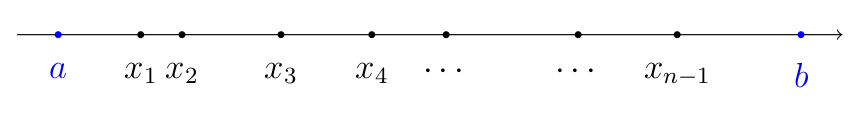
\includegraphics{./deco.png}

\begin{Definition}[Step function]
$f:[a,b]\to\mathbb{R}$ is called a~\emph{step function} if it is piecewisely constant, i.e. there exists a decomposition $\{x_{0},\ldots,x_{n}\}$ of $[a,b]$ and some $c_1,\ldots,c_n\in\mathbb{R}$ such that for all $i=1,\ldots,n$ holds
\[f(x)=c_i\text{ for all }x\in(x_{i-1},x_i).\]
The set of step functions on $[a,b]$ is denoted by $\mathcal{T}([a,b])$.
\end{Definition}

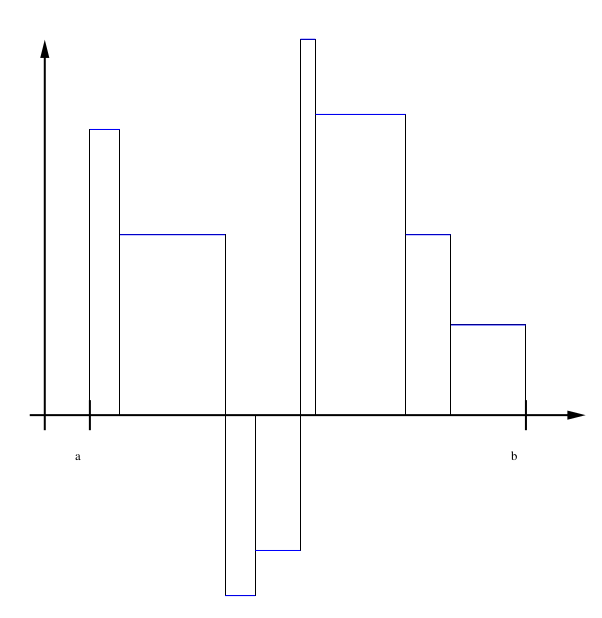
\includegraphics{./step.png}

It can be readily verified that for two step functions $f_1,f_2\in \mathcal{T}([a,b])$ holds
$f_1+f_2\in \mathcal{T}([a,b])$. As well, we have $\lambda f_1\in \mathcal{T}([a,b])$.  Hence, $\mathcal{T}([a,b])$ is a~vector space. Furthermore, since step functions only attain finitely many values, they are bounded.

%Therefore, we can conclude the following:
%\begin{lemma}
%Any step function is bounded.
%\end{lemma}

